\section{Introduction}
\label{sec:part-dina}

\subsection{Présentation du projet}
Le projet \textit{Coursidor} est un jeu stratégique inspiré du célèbre jeu de société \textit{Quoridor}, où les joueurs doivent visiter un ensemble de cases appelées \textit{objectifs} avant de revenir à leur case de départ. Deux joueurs s’affrontent dans une partie à tour de rôle. Chaque joueur peut soit se déplacer selon des règles spécifiques de direction et de distance, soit poser un mur pour ralentir son adversaire. Le jeu se déroule sur un graphe qui représente les connexions entre les différentes cases du plateau.

\subsection{État des lieux du projet}
Le projet en est actuellement à un stade où un serveur central joue un rôle crucial. Ce serveur est chargé de plusieurs tâches importantes : il charge dynamiquement les bibliothèques des joueurs, joue le premier coup et gère l’ensemble de la partie. Il sert de lien entre tous les fichiers et fonctions implémentés dans notre projet.

Chaque joueur dispose de quatre fonctions principales (\texttt{get\_player\_name}, \texttt{initialize}, \texttt{play}, \texttt{finalize}). Ces fonctions permettent aux joueurs de participer activement à la partie en utilisant des stratégies spécifiques.

En outre, un plateau de jeu a été conçu pour contenir toutes les informations sur les coups joués. Ce plateau sert de registre, enregistrant chaque mouvement et assurant le suivi de la progression de la partie. Grâce à cette structure, nous pouvons analyser les parties et améliorer les stratégies en fonction des résultats observés.


\section{Architecture modulaire}

Du point de vue de la modularité, la figure~\ref{fig:dependencies} illustre les dépendances entre les fichiers d'en-tête du projet.

\begin{figure}[H]
    \centering
    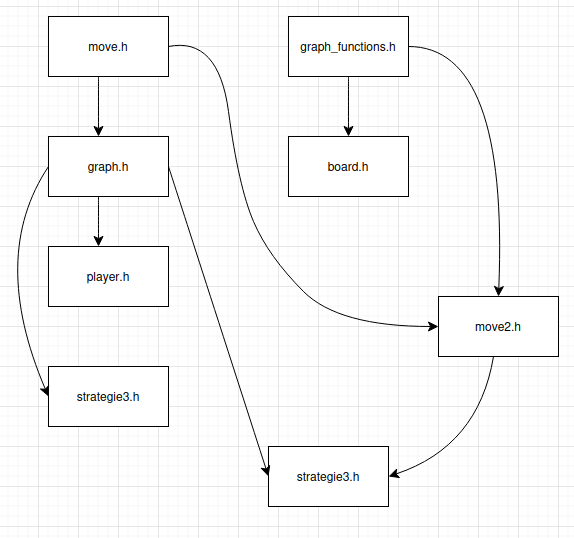
\includegraphics[width=0.45\textwidth]{rapport/draw.png} 
    \caption{Graphe des dépendances entre les fichiers d'en-tête}
    \label{fig:dependencies}
  \end{figure}

 
    \texttt{board.h} : Ce fichier regroupe les fonctions liées à la gestion du plateau de jeu, notamment l’initialisation du plateau et l’enregistrement des coups joués.\\
    \texttt{player.h} : Ce fichier contient les structures et fonctions associées à la gestion des joueurs, en particulier leurs déplacements.\\
    \texttt{move.h} : Ce fichier définit les structures fondamentales pour représenter les coups joués par les joueurs.\\
    \texttt{graph.h} : Ce fichier définit la structure de données représentant le plateau de jeu sous forme de graphe, ainsi que les types associés à sa manipulation.\\
    \texttt{graph\_functions.h} : Ce fichier assure la liaison entre la représentation géométrique graph (en coordonnées axiales pour un pavage hexagonal) et sa représentation sous forme de structure graphe qui est exploitée par les algorithmes . \\
    \texttt{strategies.h et strategie3.h}: Ces fichiers regroupent les fonctions liées aux stratégies de jeu, telles que l’algorithme de Dijkstra, A*, le TSP (problème du voyageur de commerce), la pose de murs, et les choix des mouvements intelligents du joueur.\\


Le fichier \texttt{server.c} joue un rôle central dans l’architecture du projet. Il orchestre le déroulement complet de la partie en gérant la boucle principale du jeu. Il est responsable du \textbf{chargement dynamique} des bibliothèques des joueurs à l’aide de la fonction \texttt{dlopen}, de l’initialisation du plateau de jeu, du premier coup joué, ainsi que de la validation des coups à chaque tour. Il interagit directement avec plusieurs fichiers clés, tels que \texttt{graph\_functions.h} pour la gestion du graphe, et \texttt{move2.h} pour la vérification de la validité des actions. Le serveur assure alors la cohérence du jeu, la synchronisation des états entre joueurs et la détection des conditions de victoire ou d’erreurs.
